\chapter{Implementation Details Template}
This is where you explain what you have implemented and how you have implemented it. Place here all the details that you consider important, organize the chapter in sections and subsections to explain the development and your workflow.\\Given the self-explicative title of the chapter, readers usually skip it. This is ok, because this entire chapter is simply meant to describe the details of your work so that people that are very interested (such as people who have to evaluate your work or people who have to build something more complex starting from what you did) can fully understand what you developed or implemented.\\Don't worry about placing too many details in this chapter, the only essential thing is that you keep everything tidy, without mixing too much information (so make use of sections, subsections, lists, etc.). As usual, pictures are helpful.
\chapter{Implementation Details}

\section{Overview}
In questa sezione viene fornita una panoramica generale dell'implementazione del jammer di microfoni. L'obiettivo del progetto è stato quello di disturbare i microfoni utilizzando segnali ultrasonici generati da un sistema controllato da remoto tramite Apple Home e MQTT. Di seguito sono dettagliate tutte le fasi di sviluppo, dall'hardware al software, fino alla progettazione 3D e all'integrazione finale.
In that section we will provide a detailed explanation of the implementation of the microphone jammer. The project aimed to disrupt microphones using ultrasonic signals generated by a system remotely controlled via Apple Home and MQTT.
Below are detailed all the development phases, from hardware to software, to 3D design and final integration.


\section{Hardware Setup}

\subsection{Microcontroller - Arduino Uno}
An Arduino Uno microcontroller was used to manage the system. Arduino was chosen for its ease of use and flexibility, allowing it to interface with a wide range of hardware devices. 
Below are its key technical specifications:
\begin{itemize}
    \item \textbf{Microcontroller}: ATmega328P
    \item \textbf{Operating Voltage}: 5V
    \item \textbf{Input Voltage (recommended)}: 7-12V
    \item \textbf{Input Voltage (limit)}: 6-20V
    \item \textbf{Digital I/O Pins}: 14 (6 PWM outputs)
    \item \textbf{Analog Input Pins}: 6
    \item \textbf{DC Current per I/O Pin}: 20 mA
    \item \textbf{DC Current for 3.3V Pin}: 50 mA
    \item \textbf{Flash Memory}: 32 KB (0.5 KB used by bootloader)
    \item \textbf{SRAM}: 2 KB
    \item \textbf{EEPROM}: 1 KB
    \item \textbf{Clock Speed}: 16 MHz
    \item \textbf{Interfaces}: UART, SPI, I2C
\end{itemize}
The microcontroller was employed to control the signal generator, ensuring it produced the desired waveform at the required frequency. 

\subsection{Signal Generator - AD9833}

The \textbf{AD9833} signal generator was utilized in this project to produce the ultrasonic signals required to interfere with microphones. The AD9833 is a highly versatile, low-power, programmable waveform generator that can generate \textit{sine}, \textit{triangle}, and \textit{square wave} outputs over a wide frequency range. It employs a \textbf{numerically controlled oscillator (NCO)} to ensure precise frequency generation with minimal drift, making it ideal for applications requiring stable and accurate signal production.

Key features of the AD9833 include:

\begin{itemize}
    \item \textbf{Frequency Range}: The AD9833 is capable of generating waveforms from near-DC to several MHz. In this project, it was configured to output signals in the ultrasonic range, specifically between $24 kHz$ up to $26 kHz$.
    
    \item \textbf{Low Power Consumption}: With typical power consumption of $20 mW$, the AD9833 is well-suited for battery-powered applications. Its energy efficiency made it an ideal choice for the portable jammer system developed in this project.
    
    \item \textbf{Waveform Generation}: The AD9833 can produce \textit{sine}, \textit{triangle}, and \textit{square waves}, providing flexibility in signal generation. For this project, the \textit{square wave output} was selected due to its efficiency in driving the ultrasonic transducers and maximizing interference with microphone diaphragms.
    
    \item \textbf{Programmability}: The output frequency and waveform type of the AD9833 are fully programmable via the \textbf{SPI (Serial Peripheral Interface)}. This programmability allows dynamic adjustments of the ultrasonic signal, facilitating quick testing of different frequencies to identify the optimal one for microphone disruption.
    
    \item \textbf{Compact Size}: The AD9833 is available in a small \textit{10-lead MSOP package}, which makes it ideal for compact designs. Its size made it well-suited for the jammer system, where space was limited.
\end{itemize}

In this implementation, the AD9833 was controlled by an Arduino through the SPI interface, with the output waveform subsequently amplified and transmitted via ultrasonic transducers. This configuration allowed for precise generation of high-frequency signals that were capable of effectively disrupting nearby microphones.

\subsection{SPI Communication Protocol}

The AD9833 programmable waveform generator communicates with the Arduino Uno using the SPI (Serial Peripheral Interface) protocol. SPI is a synchronous serial communication protocol commonly used to exchange data between a master device (in this case, the Arduino) and one or more slave devices (such as the AD9833). The protocol is fast and efficient, utilizing four main signals:

\begin{itemize}
    \item \textbf{MOSI (Master Out Slave In)}: Sends data from the master (Arduino) to the slave (AD9833).
    \item \textbf{MISO (Master In Slave Out)}: Receives data from the slave. (Not used in this specific application with the AD9833.)
    \item \textbf{SCLK (Serial Clock)}: Synchronizes the communication by generating clock pulses.
    \item \textbf{SS/CS (Slave Select/Chip Select)}: Selects which slave device is active for communication.
\end{itemize}

In this project, only three of these signals are needed, as the AD9833 is a write-only device, meaning that it does not send data back to the master.

SPI operates by shifting data in or out of the slave device one bit at a time, synchronized by the clock signal. The data is sent over the \textbf{MOSI} line, with the clock signal driving the data transfer, and the \textbf{SS/CS} line controlling when the slave device (AD9833) is selected for communication.

\subsection{Pin Configuration for AD9833 Communication}

Below are the specific pin configurations used to connect the AD9833 with the Arduino Uno via SPI:

\subsubsection{FSYNC (SS/CS) – Pin 10}
\begin{verbatim}
#define AD9833_FSYNC 10  // PIN SS/CS
\end{verbatim}

The FSYNC pin is assigned to Pin 10 on the Arduino and serves as the \textit{Slave Select (SS)} or \textit{Chip Select (CS)} pin. The FSYNC pin determines when the AD9833 is selected and ready for communication.

\begin{itemize}
    \item When the FSYNC pin is set to \textbf{LOW}, the AD9833 is selected and activated for communication.
    \item When the FSYNC pin is set to \textbf{HIGH}, the AD9833 is deselected and no communication occurs.
\end{itemize}

\subsubsection{SCLK (SCK) – Pin 13}
\begin{verbatim}
#define AD9833_SCLK 13   // PIN SCK
\end{verbatim}

The SCLK pin is defined as the \textit{Serial Clock (SCK)} and is connected to Pin 13 on the Arduino. It generates the clock pulses that synchronize the data transfer between the Arduino and the AD9833.

\begin{itemize}
    \item For every clock pulse on the SCLK line, one bit of data is transmitted or received.
    \item The clock signal ensures that both the Arduino and the AD9833 are synchronized during data transmission.
\end{itemize}

\subsubsection{FDATA (MOSI) – Pin 11}
\begin{verbatim}
#define AD9833_FDATA 11  // PIN MOSI
\end{verbatim}

The FDATA pin is connected to Pin 11 on the Arduino and serves as the \textit{Master Out Slave In (MOSI)} pin. It is used to transmit data from the Arduino to the AD9833.

\begin{itemize}
    \item Configuration data and waveform instructions are transmitted from the Arduino to the AD9833 via the MOSI line.
    \item Data is sent sequentially, one bit at a time, in synchronization with the clock pulses on the SCLK line.
\end{itemize}

\subsection{Summary of Pin Roles in SPI for AD9833}

\begin{itemize}
    \item \textbf{FSYNC (Pin 10)}: Acts as the \textit{Slave Select (SS/CS)} pin to activate or deactivate the AD9833 for communication.
    \item \textbf{SCLK (Pin 13)}: Provides the \textit{Serial Clock (SCK)} signal, ensuring synchronized data transfer between the Arduino and AD9833.
    \item \textbf{FDATA (Pin 11)}: Serves as the \textit{Master Out Slave In (MOSI)} pin, transmitting data from the Arduino to the AD9833.
\end{itemize}

This pin configuration allows precise control of the AD9833 using SPI communication, facilitating the generation of the required waveforms at the desired frequency.

\subsection{Ultrasound Transducers}

The ultrasonic transducers used in this project operate at a frequency of $20 \text{kHz}$, which is beyond the audible range for humans. These transducers are particularly effective for disrupting microphones, as they generate high-frequency sound waves that induce vibrations in the microphone diaphragm, impairing its ability to capture sound accurately.

To maximize the interference effect, the placement and orientation of the transducers are crucial. The transducers should be positioned in close proximity to the target microphones and aligned to ensure the ultrasonic waves are directed precisely at the microphones. One key factor influencing the effectiveness of this interference is the beam angle of the transducers, which defines the spread of the ultrasonic waves.

The beam angle determines how focused or dispersed the sound waves are as they propagate. A narrower beam angle results in a more concentrated sound wave, which can enhance the interference effect over longer distances, while a wider beam angle covers a broader area but with less intensity. Given these considerations, both theoretical and empirical analyses were conducted to identify the optimal arrangement of the transducer array, accounting for beam angle, proximity, and orientation to achieve the most effective disruption of microphone performance.
\begin{figure}[h!]
    \centering
    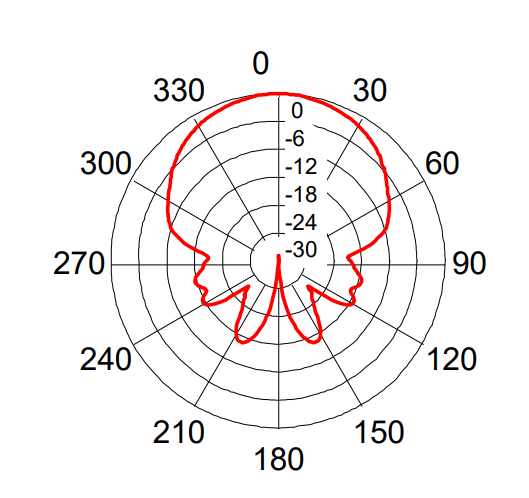
\includegraphics[width=0.5\textwidth]{images/Beam_Angle.png}
    \caption{Beam Angle}
    \label{fig:transducer_shape}
\end{figure}

\subsection{Amplifier - TPA3116D2}

The ultrasonic signals generated by the AD9833, controlled via the Arduino, are amplified using the \textbf{TPA3116D2}, a high-efficiency, Class D audio amplifier from Texas Instruments. The amplifier ensures that the ultrasonic transducers receive a sufficiently powerful signal to produce sound waves with the necessary intensity for effective microphone interference.

The \textbf{TPA3116D2} is specifically designed for high-performance audio applications and is capable of delivering output power of up to \textit{50 W} per channel (with a 4 $\Omega$ load). Key features of the \textbf{TPA3116D2} that make it suitable for this project include:

\begin{itemize}
    \item \textbf{High Efficiency}: The Class D architecture of the amplifier provides high efficiency, with typical values reaching \textit{90\%}. This reduces heat dissipation and ensures lower power consumption, making it well-suited for applications where energy efficiency is critical.
    
    \item \textbf{Output Power}: The TPA3116D2 can deliver up to $50 W$ per channel in stereo mode, or $100 W$ in mono mode. In this project, the amplifier was used to boost the signal to a level that could drive the ultrasonic transducers effectively, ensuring a strong and clear output at the target frequency of \textit{20 kHz}.
    
    \item \textbf{Low Distortion and Noise}: The amplifier features a low distortion rate, typically less than \textit{0.1\% Total Harmonic Distortion + Noise (THD+N)} at full power, ensuring that the signal remains clean. This is crucial for maintaining the integrity of the ultrasonic signal being transmitted to the transducers, as distortion could reduce the effectiveness of the interference.
    
    \item \textbf{Thermal and Overcurrent Protection}: The \textbf{TPA3116D2} includes built-in thermal and overcurrent protection, ensuring reliable operation even under high-power conditions. This feature enhances the robustness of the system, especially when used in a continuous mode, as is typical in ultrasonic jamming applications.
    
    \item \textbf{Wide Supply Voltage Range}: The amplifier operates across a wide supply voltage range of \textit{4.5 V to 26 V}, providing flexibility in power supply options. In this project, the TPA3116D2 was powered using a suitable DC supply to ensure adequate power delivery to the transducers.
    
\end{itemize}

The amplified ultrasonic signals were then fed into the ultrasonic transducers, which required a sufficiently strong input to generate the desired high-frequency output. The use of the \textbf{TPA3116D2} allowed for an efficient and powerful amplification stage, ensuring that the transducers operated at optimal levels to effectively disrupt nearby microphones.


\subsection{Power Supply}
\subsection{Power Supply}

The system is powered by a set of rechargeable lithium-ion batteries. The selection of these batteries was made considering the total power consumption of the system, which includes the Arduino, the TPA3116D2 amplifier, and the ESP8266 Wi-Fi module.

The batteries are characterized by the following specifications:

\begin{itemize}
    \item \textbf{Nominal Voltage}: \textit{3.7 V}
    \item \textbf{Capacity}: \textit{2600 mAh}
    \item \textbf{Maximum Discharge Current}: \textit{3 A} (Continuous)
\end{itemize}

These batteries were chosen for the following reasons:
\begin{itemize}
    \item \textbf{Portability}: The compact size and rechargeable nature of the lithium-ion cells ensure that the system remains portable and easy to use in various settings.
    \item \textbf{Extended Operation}: With a capacity of \textit{2600 mAh}, these batteries provide a substantial amount of energy, allowing the system to operate for extended periods between charges.
    \item \textbf{Stable Voltage Supply}: The nominal voltage of \textit{3.7 V} is suitable for powering the ESP8266 module and can be regulated to meet the voltage requirements of the Arduino and amplifier.
    \item \textbf{High Discharge Current Capability}: The maximum discharge current of \textit{3 A} ensures that the batteries can handle the peak currents required by the TPA3116D2 amplifier during operation.
\end{itemize}

The use of batteries ensures reliable power supply, contributing to the overall portability and efficiency of the system. Their high energy density and stable performance make them an ideal choice for this application.

\subsection{ESP8266}

For remote control of the jammer, the \textbf{ESP8266} Wi-Fi module was employed. This module connects to a local Wi-Fi network and is configured to receive commands via the MQTT protocol and Apple HomeKit, enabling control of the jammer's operation from a mobile device or other connected clients.

The \textbf{ESP8266} is a low-cost, highly-integrated Wi-Fi microchip designed for a variety of wireless communication applications. Its key features include:

\begin{itemize}
    \item \textbf{Built-in Wi-Fi Connectivity}: The ESP8266 includes an integrated 2.4 GHz Wi-Fi transceiver, providing reliable wireless communication. It supports the IEEE 802.11 b/g/n Wi-Fi standards, ensuring compatibility with most Wi-Fi networks.
    
    \item \textbf{Processing Power}: The module is equipped with a 32-bit RISC processor, running at up to \textit{160 MHz}, and includes built-in memory, which supports the execution of complex tasks and protocols directly on the module.
    
    \item \textbf{Flexible Communication Protocols}: The ESP8266 supports multiple communication protocols, including TCP/IP, UDP, HTTP, and MQTT. In this project, MQTT was used to facilitate communication between the module and the remote control interface.
    
    \item \textbf{Integration with Apple HomeKit}: The ESP8266 was configured to work with Apple HomeKit, enabling seamless integration into the Apple ecosystem. This setup allows the jammer to be controlled using Apple's Home app or via Siri voice commands.
    
    \item \textbf{Low Power Consumption}: The module supports various power-saving modes, making it suitable for battery-operated applications. It can operate efficiently in both active and sleep modes, contributing to the overall energy efficiency of the system.
    
    \item \textbf{GPIO Pins and Interfaces}: The ESP8266 features multiple General Purpose Input/Output (GPIO) pins that can be used for interfacing with external hardware, such as sensors and actuators. For this project, GPIO pins were used to control the power to the jammer.
\end{itemize}

The ESP8266 was configured to connect to a local Wi-Fi network and receive commands via MQTT messages. This setup allows users to remotely manage the jammer, turning it on or off through a mobile device or other networked clients. The integration with Apple HomeKit further enhances usability, providing a user-friendly interface for controlling the system.

\subsection{SRD-05VDC-SL-C Relay Module}

To control the power supply of the jammer, an \textbf{SRD-05VDC-SL-C} relay module was used. This relay module is a key component in switching the high-power signals required for the ultrasonic transducers and other parts of the system.

The \textbf{SRD-05VDC-SL-C} is a general-purpose electromagnetic relay with the following features:

\begin{itemize}
    \item \textbf{Coil Voltage}: The relay operates with a coil voltage of \textit{5 V DC}, which is compatible with the voltage levels provided by the ESP8266 and other control circuits in the system.
    
    \item \textbf{Contact Configuration}: It has a Single Pole Double Throw (SPDT) configuration, which includes one common contact (COM), one normally open contact (NO), and one normally closed contact (NC). This allows for versatile switching applications, enabling the relay to connect or disconnect the power supply to the jammer as required.
    
    \item \textbf{Maximum Switching Current}: The relay can handle up to \textit{10 A} at \textit{250 V AC} or \textit{30 V DC}, making it suitable for switching relatively high currents and voltages used in the jammer system.
    
    \item \textbf{Contact Material}: The contacts are made of Silver Alloy (AgSnO\(_2\)), which provides durability and resistance to electrical arcing, ensuring reliable operation over time.
    
    \item \textbf{Physical Size}: The relay is compact, with dimensions of approximately \textit{29 mm x 12.5 mm x 23 mm}, making it easy to integrate into various circuit designs.
    
    \item \textbf{LED Indicator}: The module includes an onboard LED indicator that illuminates when the relay is activated, providing a visual confirmation of its status.
\end{itemize}

In this project, the \textbf{SRD-05VDC-SL-C} relay is mounted on a dedicated adapter board designed for the ESP8266. This adapter board simplifies the connection between the relay and the ESP8266 by providing appropriate pin mappings and necessary connections. The relay module is used to control the power supply to the jammer, allowing the ESP8266 to switch the jammer on or off remotely. 

The relay's high current handling capability ensures that it can manage the power requirements of the jammer's circuitry safely and effectively. Its integration into the project helps in achieving reliable and controlled operation of the system.


\section{Software Development}

In this section, we will analyze the software code used in the project in detail. The software development process encompasses the creation of the code to control the AD9833 signal generator and the TPA3116D2 amplifier, as well as the integration of the ESP8266 for remote control. The following subsections provide a comprehensive overview of the code structure, libraries used, and key functionalities implemented.

\subsection{Arduino Source Code}

The Arduino source code is responsible for controlling the signal generation and amplification components of the system. The code is written in \textit{C++} using the Arduino Integrated Development Environment (IDE). It utilizes specific libraries to facilitate communication and control:

\subsubsection{Libraries Used}
\begin{itemize}
    \item \texttt{SPI.h}: This library provides the necessary functions for SPI communication, which is essential for interfacing with the AD9833 signal generator.
    \item \texttt{AD9833.h} by Rob Tillart: This library simplifies the management of the AD9833 signal generator by abstracting the low-level SPI commands into high-level functions.
\end{itemize}

\subsubsection{Code Overview}
The code begins with the inclusion of necessary libraries and the definition of pin configurations. The key components of the code are as follows:

\begin{itemize}
    \item \textbf{Initialization}: The code initializes the serial communication for debugging and sets up the AD9833 signal generator using the \texttt{AD9833.begin()} function.
    \item \textbf{Waveform Configuration}: The waveform type is set to a square wave using \texttt{ad9833.setWave(AD9833\_SQUARE1)}, and the initial phase is configured to zero.
    \item \textbf{Frequency Sweeping}: In the main loop, the code performs a frequency sweep by iterating through a predefined set of values. These values are read from program memory (PROGMEM) and used to adjust the output frequency of the AD9833.
\end{itemize}

\begin{verbatim}
#include <SPI.h>
#include <AD9833.h>
#include <avr/pgmspace.h>

// Pin di connessione per AD9833
#define AD9833_FSYNC 10  // PIN SS/CS

// Crea un oggetto AD9833
AD9833 ad9833(AD9833_FSYNC);

// Valori randomizzati per lo sweep tra 24kHz e 26kHz
const uint8_t randomized[] PROGMEM = { /* valori qui */ };

void setup() {
    // Inizializza la comunicazione seriale per il debug
    Serial.begin(9600);
    Serial.println("AD9833 Sweep Test");

    // Inizializza il generatore di segnale AD9833
    ad9833.begin();

    // Imposta la modalità d'onda a onda quadra
    ad9833.setWave(AD9833_SQUARE1); // Modalità onda quadra (divisa per 2)
    ad9833.setPhase(0);                      // Imposta la fase iniziale a 0
}

void loop() {
    // Effettua lo sweep tra 24kHz e 26kHz con valori randomizzati
    for (uint16_t i = 0; i < sizeof(randomized); i++) {
        // Leggi il valore randomizzato dalla memoria PROGMEM
        uint8_t rand_val = pgm_read_byte_near(randomized + i);
        
        // Imposta la frequenza di output (da 24000Hz a 26000Hz)
        ad9833.setFrequency(24000 + rand_val, 0);

        delay(100);
    }
}
\end{verbatim}


\subsection{ESP8266 Code}

The ESP8266 module is used to enable remote control of the jammer via a Wi-Fi network. The provided code implements both MQTT and Apple HomeKit protocols to facilitate this control. Below is an overview of the key components and functionalities of the ESP8266 code.

\subsubsection{Libraries and Configuration}

The ESP8266 code uses several libraries to handle Wi-Fi connectivity, MQTT communication, and HomeKit integration:
\begin{itemize}
    \item \texttt{ESP8266WiFi.h}: Handles Wi-Fi connectivity.
    \item \texttt{PubSubClient.h}: Manages MQTT communication.
    \item \texttt{Arduino.h}: Provides standard Arduino functions.
    \item \texttt{arduino\_homekit\_server.h}: Manages HomeKit functionalities.
    \item \texttt{wifi\_info.h}: Contains Wi-Fi credentials and connection functions.
\end{itemize}

\subsubsection{Code Overview}

\paragraph{Global Definitions and Initialization}
The ESP8266 is configured with the MQTT broker address and initializes both Wi-Fi and MQTT clients.

\begin{verbatim}
const char* mqtt_server = "broker.hivemq.com";
WiFiClient espClient;
PubSubClient client(espClient);
#define PIN_LED 0 
\end{verbatim}

\paragraph{Callback Function}
The \texttt{callback()} function processes incoming MQTT messages. It toggles an LED based on the received message and updates the HomeKit state.

\begin{verbatim}
void callback(char* topic, byte* payload, unsigned int length) {
    Serial.print("Message received on topic: ");
    Serial.println(topic);

    String payloadStr;
    for (unsigned int i = 0; i < length; i++) {
        payloadStr += (char)payload[i];
    }

    if (strcmp(topic, "CosFraGia/JammerProject") == 0) {
        if (payloadStr == "Accendi") {
            digitalWrite(PIN_LED, HIGH);  // Turn on
            cha_switch_on.value.bool_value = false;  // Update HomeKit state
        } else if (payloadStr == "Spegni") {
            digitalWrite(PIN_LED, LOW);   // Turn off
            cha_switch_on.value.bool_value = true;  // Update HomeKit state
        }
        homekit_characteristic_notify(&cha_switch_on, cha_switch_on.value);  // Notify HomeKit
    }
}
\end{verbatim}

\paragraph{MQTT Reconnection}
The \texttt{reconnect()} function ensures that the ESP8266 maintains a connection to the MQTT broker. It attempts to reconnect if the connection is lost.

\begin{verbatim}
void reconnect() {
    while (!client.connected()) {
        if (client.connect("ArduinoClient")) {
            client.subscribe("CosFraGia/JammerProject");
        } else {
            delay(5000);
        }
    }
}
\end{verbatim}

\paragraph{Wi-Fi Setup}
The \texttt{setup\_wifi()} function connects the ESP8266 to the specified Wi-Fi network and prints the IP address upon successful connection.

\begin{verbatim}
void setup_wifi() {
    WiFi.begin(ssid, password);
    while (WiFi.status() != WL_CONNECTED) {
        delay(500);
    }
    Serial.println("WiFi connected");
    Serial.println("IP Address: ");
    Serial.println(WiFi.localIP());
}
\end{verbatim}

\paragraph{Setup and Loop Functions}
In the \texttt{setup()} function, serial communication, Wi-Fi connection, HomeKit setup, and MQTT client configuration are initialized. The \texttt{loop()} function manages HomeKit interactions and maintains the MQTT connection.

\begin{verbatim}
void setup() {
    Serial.begin(115200);
    pinMode(PIN_LED, OUTPUT);
    wifi_connect(); // from wifi_info.h
    my_homekit_setup();
    client.setServer(mqtt_server, 1883);
    client.setCallback(callback);
}

void loop() {
    my_homekit_loop();
    if (!client.connected()) {
        reconnect();
    }
    client.loop();
    delay(10);
}
\end{verbatim}

\paragraph{HomeKit Integration}
The HomeKit setup and loop functions configure the HomeKit server and handle switch events. The \texttt{cha\_switch\_on\_setter()} function updates the switch state based on HomeKit commands.

\begin{verbatim}
void cha_switch_on_setter(const homekit_value_t value) {
    bool on = value.bool_value;
    cha_switch_on.value.bool_value = on;  // Sync the value
    digitalWrite(PIN_SWITCH, on ? LOW : HIGH);
}

void my_homekit_setup() {
    pinMode(PIN_SWITCH, OUTPUT);
    digitalWrite(PIN_SWITCH, HIGH);
    cha_switch_on.setter = cha_switch_on_setter;
    arduino_homekit_setup(&config);
}

void my_homekit_loop() {
    arduino_homekit_loop();
}
\end{verbatim}

\paragraph{Accessory Definition}
The accessory is defined using the HomeKit library, including characteristics such as the switch state and accessory information.

\begin{verbatim}
homekit_characteristic_t cha_switch_on = HOMEKIT_CHARACTERISTIC_(ON, false);
homekit_characteristic_t cha_name = HOMEKIT_CHARACTERISTIC_(NAME, "Switch");

homekit_accessory_t *accessories[] = {
    HOMEKIT_ACCESSORY(.id=1, .category=homekit_accessory_category_switch, .services=(homekit_service_t*[]) {
        HOMEKIT_SERVICE(ACCESSORY_INFORMATION, .characteristics=(homekit_characteristic_t*[]) {
            HOMEKIT_CHARACTERISTIC(NAME, "Jammer"),
            HOMEKIT_CHARACTERISTIC(MANUFACTURER, "Arduino HomeKit"),
            HOMEKIT_CHARACTERISTIC(SERIAL_NUMBER, "1112233"),
            HOMEKIT_CHARACTERISTIC(MODEL, "CostaBot"),
            HOMEKIT_CHARACTERISTIC(FIRMWARE_REVISION, "1.0"),
            HOMEKIT_CHARACTERISTIC(IDENTIFY, my_accessory_identify),
            NULL
        }),
        HOMEKIT_SERVICE(SWITCH, .primary=true, .characteristics=(homekit_characteristic_t*[]){
            &cha_switch_on,
            &cha_name,
            NULL
        }),
        NULL
    }),
    NULL
};

homekit_server_config_t config = {
    .accessories = accessories,
    .password = "121-33-772"
};
\end{verbatim}

This section provides an in-depth analysis of the ESP8266 code, highlighting how it integrates with MQTT and HomeKit to manage remote control of the jammer. The code demonstrates how the ESP8266 handles Wi-Fi connectivity, MQTT messaging, and HomeKit interactions to enable versatile control options.

\section{Assembly and Integration}

\subsection{Physical Assembly}
Dopo la stampa 3D, tutti i componenti hardware sono stati assemblati all'interno del case stampato. Le connessioni tra Arduino, amplificatore, transducer e modulo Wi-Fi sono state effettuate seguendo uno schema di cablaggio preciso per minimizzare interferenze e problemi di spazio.

\subsection{Testing and Calibration}
Il sistema è stato testato per garantire la corretta emissione dei segnali ultrasonici. La calibrazione è stata necessaria per regolare la frequenza del segnale
